\documentclass[svgnames,portrait,final,usenames,dvipsnames]{baposter}
%\documentclass[a4shrink,portrait,final]{baposter}
% Usa a4shrink for an a4 sized paper.

\tracingstats=2

%% Language and babel
\usepackage[utf8]{inputenc}
\usepackage[T1]{fontenc}
\usepackage[english,french,italian]{babel}

\usepackage{mdwlist}
\usepackage{times}
\usepackage{calc}
\usepackage{relsize}
\usepackage{multirow}
\usepackage{bm}

% Math
\usepackage{siunitx}

%% Images
\usepackage{float}
\usepackage{graphicx}
\usepackage{wrapfig}
\usepackage{cclicenses}
\usepackage{sidecap}
\usepackage[font=scriptsize,labelfont=bf]{caption}

%% tikz
\usepackage[]{xcolor}
\usepackage{tikz}
\usetikzlibrary{shapes,arrows}
\usepackage{rotating}

%% Layout
\usepackage{multicol}
\usepackage{pgfbaselayers}
\pgfdeclarelayer{background}
\pgfdeclarelayer{foreground}
\pgfsetlayers{background,main,foreground}

\usepackage{helvet}
\usepackage{palatino}

\selectcolormodel{cmyk}

\graphicspath{{../source/img/}}

%% [biblatex] introduzione pacchetti utili per BibLaTeX
\usepackage[babel]{csquotes}
\usepackage[babel=hyphen,hyperref,backend=biber]{biblatex}

\addbibresource{../source/refs/bibliografia.bib}

%%%%%%%%%%%%%%%%%%%%%%%%%%%%%%%%%%%%%%%%%%%%%%%%%%%%%%%%%%%%%%%%%%%%%%%%%%%%%%%%
% Multicol Settings
%%%%%%%%%%%%%%%%%%%%%%%%%%%%%%%%%%%%%%%%%%%%%%%%%%%%%%%%%%%%%%%%%%%%%%%%%%%%%%%%
\setlength{\columnsep}{0.8em}
\setlength{\columnseprule}{0mm}

%%%%%%%%%%%%%%%%%%%%%%%%%%%%%%%%%%%%%%%%%%%%%%%%%%%%%%%%%%%%%%%%%%%%%%%%%%%%%%%%%
%% Save space in lists. Use this after the opening of the list
%%%%%%%%%%%%%%%%%%%%%%%%%%%%%%%%%%%%%%%%%%%%%%%%%%%%%%%%%%%%%%%%%%%%%%%%%%%%%%%%%
\newcommand{\compresslist}{%
\setlength{\itemsep}{1pt}%
\setlength{\parskip}{0pt}%
\setlength{\parsep}{0pt}%
}

%%%%%%%%%%%%%%%%%%%%%%%%%%%%%%%%%%%%%%%%%%%%%%%%%%%%%%%%%%%%%%%%%%%%%%%%%%%%%%%%
% CORREZIONI DI STILE %
%%%%%%%%%%%%%%%%%%%%%%%%%%%%%%%%%%%%%%%%%%%%%%%%%%%%%%%%%%%%%%%%%%%%%%%%%%%%%%%%

%% aggiunge una virgola tra Autore e anno nello stile citazione authoryear
\renewcommand{\nameyeardelim}{, } % this doesn't work anymore

%% sostituisce le parentesi tonde dell'anno di pubblicazione con "niente"
\renewcommand{\bibleftparen}{}
\renewcommand{\bibrightparen}{}

%% separa gli elementi della citazione con una virgola anzichè i punti
\renewcommand*{\newunitpunct}{\addcomma\space}

%% rende corsivo il titolo dell'articolo
\DeclareFieldFormat[article]{title}{\mkbibemph{#1}}

%% aggiunge "«»" al nome del giornale di pubblicazione, e fa seguire da una virgola
\DeclareFieldFormat{journaltitle}{\guillemotleft{#1}\guillemotright ,}
\DeclareFieldFormat{pages}{{#1}}

%% rende smallcapitals i nomi degli autori nella citazione
\renewcommand*{\mkbibnamelast}[1]{%
    \ifmknamesc{\textsc{#1}}
}

%%%%%%%%%%%%%%%%%%%%%%%%%%%%%%%%%%%%%%%%%%%%%%%%%%%%%%%%%%%%%%%%%%%%%%%%%%%%%%
%%% Begin of Document
%%%%%%%%%%%%%%%%%%%%%%%%%%%%%%%%%%%%%%%%%%%%%%%%%%%%%%%%%%%%%%%%%%%%%%%%%%%%%%

\begin{document}

%%%%%%%%%%%%%%%%%%%%%%%%%%%%%%%%%%%%%%%%%%%%%%%%%%%%%%%%%%%%%%%%%%%%%%%%%%%%%%
%%% Here starts the poster
%%%---------------------------------------------------------------------------
%%% Format it to your taste with the options
%%%%%%%%%%%%%%%%%%%%%%%%%%%%%%%%%%%%%%%%%%%%%%%%%%%%%%%%%%%%%%%%%%%%%%%%%%%%%%
% Define some colors
\definecolor{silver}{cmyk}{0,0,0,0.3}
\definecolor{yellow}{cmyk}{0,0,0.9,0.0}
\definecolor{reddishyellow}{cmyk}{0,0.22,1.0,0.0}
\definecolor{black}{cmyk}{0,0,0.0,1.0}
\definecolor{darkYellow}{cmyk}{0,0,1.0,0.5}
\definecolor{darkSilver}{cmyk}{0,0,0,0.1}

\definecolor{lightyellow}{cmyk}{0,0,0.3,0.0}
\definecolor{lighteryellow}{cmyk}{0,0,0.1,0.0}
\definecolor{lighteryellow}{cmyk}{0,0,0.1,0.0}
\definecolor{lightestyellow}{cmyk}{0,0,0.05,0.0}

%%
\typeout{Poster Starts}
\background{
    \begin{tikzpicture}[remember picture,overlay]%
        \draw (current page.north west)+(-2em,2em) node[anchor=north west] {
\includegraphics[height=1.1\textheight]{silhouettes_background}};
    \end{tikzpicture}%
}

\newlength{\leftimgwidth}
\begin{poster}%
    {% Poster Options
        grid=no,                    % Show grid to help with alignment
        colspacing=1em,             % Column spacing
        bgColorOne=lighteryellow,   % Color style
        bgColorTwo=lightestyellow,
        borderColor=reddishyellow,
        headerColorOne=yellow,
        headerColorTwo=reddishyellow,
        headerFontColor=black,
        boxColorOne=lightyellow,
        boxColorTwo=lighteryellow,
        textborder=roundedleft,     % Format of textbox
        eyecatcher=no,              % Format of text header
        headerborder=open,
        headerheight=0.08\textheight,
        headershape=roundedright,
        headershade=plain,
        headerfont=\Large\textsf,   % Sans Serif
        boxshade=plain,
        background=plain,           % background=shade-tb,
        linewidth=2pt
    }
    %%%% Eye Catcher
    % No eye catcher for this poster. (eyecatcher=no above). If an eye catcher is present, the title is centered between eye-catcher and logo.
    {\includegraphics[width=10em]{D1077}} 
    %%%% Title
    {\sf \LARGE %Sans Serif
        %\bf% Serif
        WebGIS e divulgazione del dato archeologico\\
        con software open source
    }
    %%%% Authors
    {\sf \large%Sans Serif
    % Serif
    \vspace{1em}Francesco de Virgilio, Patrizia Albrizio, Ginevra Panzarino, Enrica Zambetta \\
    \small{O.I.A. --- Open Idea for Archaeology | info@openoia.org}

    }
    %%%% University logo
    {% The makebox allows the title to flow into the logo, this is a hack because of the L shaped logo.
        \makebox[10em][r]{%
          \begin{minipage}{19em}
            \hfill
            
\includegraphics[height=7.0em]{logo}
            \hspace{0.5cm}
            
\includegraphics[height=7.0em]{logogenerale}
          \end{minipage}
        }
    }

    \tikzstyle{light shaded}=[top color=baposterBGtwo!30!white,bottom color=baposterBGone!30!white,shading=axis,shading angle=30]

    % Width of left inset image
     \setlength{\leftimgwidth}{0.78em+8.0em}

    %%%%%%%%%%%%%%%%%%%%%%%%%%%%%%%%%%%%%%%%%%%%%%%%%%%%%%%%%%%%%%%%%%%%%%%%%%%%%%
    %%% Now define the boxes that make up the poster
    %%%---------------------------------------------------------------------------
    %%% Each box has a name and can be placed absolutely or relatively.
    %%% The only inconvenience is that you can only specify a relative position 
    %%% towards an already declared box. So if you have a box attached to the 
    %%% bottom, one to the top and a third one which should be in between, you 
    %%% have to specify the top and bottom boxes before you specify the middle 
    %%% box.
    %%%%%%%%%%%%%%%%%%%%%%%%%%%%%%%%%%%%%%%%%%%%%%%%%%%%%%%%%%%%%%%%%%%%%%%%%%%%%%

    % A coloured circle useful as a bullet with an adjustably strong filling
    \newcommand{\colouredcircle}[1]{%
        \tikz{\useasboundingbox (-0.2em,-0.32em) rectangle(0.2em,0.32em); \draw[draw=black,fill=baposterBGone!80!black!#1!white,line width=0.03em] (0,0) circle(0.18em);}
    }

    %%%%%%%%%%%%%%%%%%%%%%%%%%%%%%%%%%%%%%%%%%%%%%%%%%%%%%%%%%%%%%%%%%%%%%%%%%%%%%
    \headerbox{Il caso di studio}{name=case,column=0,row=0}{\scriptsize
    %%%%%%%%%%%%%%%%%%%%%%%%%%%%%%%%%%%%%%%%%%%%%%%%%%%%%%%%%%%%%%%%%%%%%%%%%%%%%%

        Siponto (Manfredonia -- Foggia) è un'antica colonia romana dedotta nel II sec. a.C., precoce diocesi della \emph{II regio Apulia et Calabria} e fiorente porto sull'Adriatico fino all'epoca dell'abbandono, decretato dal sovrano svevo Manfredi nel 1263. 

        L'indagine sulla città si inserisce nell'ambito del programma di ricerca su \emph{Siponto. Una città portuale abbandonata}, realizzato grazie alla collaborazione istituzionale della Cattedra di Archeologia Medievale dell'Università di Bari Aldo Moro con la Soprintendenza dei Beni Archeologici della Puglia, la provincia di Foggia (Museo del Territorio), il Dipartimento di Scienze della Terra e Geoambientali dell'Università di Bari e l'Università del Salento (Laboratorio di Topografia Antica e Fotogrammetria del Dipartimento di Beni Culturali). 

        L'attività di ricerca multidisciplinare condotta a Siponto, iniziata nel 2001 e tutt'ora in corso, continua a rivelare la complessa vicenda insediativa del centro dauno nell'area ad ovest della ferrovia Foggia-Manfredonia, vicino al tratto settentrionale della cinta muraria in luce (si estende su una superficie complessiva di circa 1100 \si{\meter\squared}).

    \vspace{0.3em}
    }

    %%%%%%%%%%%%%%%%%%%%%%%%%%%%%%%%%%%%%%%%%%%%%%%%%%%%%%%%%%%%%%%%%%%%%%%%%%%%%%
    \headerbox{Il progetto}{name=project,column=0,below=case}{\scriptsize
    %%%%%%%%%%%%%%%%%%%%%%%%%%%%%%%%%%%%%%%%%%%%%%%%%%%%%%%%%%%%%%%%%%%%%%%%%%%%%%

        Il progetto ``Siponto Aperta: nuove tecnologie per la divulgazione dei beni culturali'' è stato realizzato tramite un finanziamento della Regione Puglia nell'ambito del progetto ``Bollenti Spiriti --- Principi Attivi 2010'', conclusosi formalmente nell'ottobre 2012, con la collaborazione della Cattedra di Archeologia Medievale e del Centro Interdipartimentale Strutture di Museologia Scientifica Unversitaria dell'Università degli Studi di Bari --- Aldo Moro nelle figure rispettivamente della prof.ssa Caterina Laganara e del dott. Ruggero Francescangeli. Il gruppo di lavoro si è costituito nell'associazione \emph{O.I.A. --- Open Idea for Archaeology}.

        Il progetto è stato incentrato sull'informatizzazione dei dati di scavo archeologico del sito di Siponto da realizzarsi interamente con software libero; si è cercato di rendere moderna e innovativa la gestione del \textit{workflow} di ricerca archeologica con un occhio di riguardo alla fruizione attraverso canali multimediali e innovativi, rendendo di conseguenza più efficienti i servizi destinati agli utenti.\linebreak

        Il Parco Archeologico è stato recentemente riorganizzato e aggiornato grazie all'intervento della Soprintendenza per i Beni Archeologici della Puglia, della Regione Puglia e dell'Università degli Studi di Bari. Tra le \textbf{criticità} ancora vive del sito, ricordiamo:

        \begin{itemize}
            \itemsep0em
            \item la difficoltà nell'attirare visitatori 
            \item la scarsa visibilità e leggibilità delle strutture 
            \item la totale assenza di documentazione digitale per la conoscenza e lo studio del sito (in dieci anni di lavori sono state prodotte più di 700 schede US e relative piante e sezioni)
        \end{itemize}

    Il progetto si è posto i seguenti \textbf{obiettivi}:

        \begin{itemize}
            \itemsep0em
            \item digitalizzazione della documentazione di scavo, finora quasi completamente cartacea;
            \item realizzazione di modelli 3D di alcuni tra i reperti più significativi rinvenuti;
            \item realizzazione di un sito web dalla forte impronta turistica (\textit{webtour} e ricostruzioni virtuali);
            \item implementazione di una interfaccia web per l'interrogazione del database archeologico;
            \item un webGIS per la visualizzazione dei dati stratigrafici e delle relative schede catalografiche;
            \item l'utilizzo esclusivo di software \textit{open source} di ogni singola parte del progetto e la conseguente pubblicazione del codice sorgente con licenza libera.
        \end{itemize}
        %\vspace{0.3em}
    }

    %%%%%%%%%%%%%%%%%%%%%%%%%%%%%%%%%%%%%%%%%%%%%%%%%%%%%%%%%%%%%%%%%%%%%%%%%%%%%%
    \headerbox{WebGIS archeologici: stato dell'arte di \emph{frontend} e \emph{backend}}{name=webgis-status,column=1,span=2,row=0}{\scriptsize
    %%%%%%%%%%%%%%%%%%%%%%%%%%%%%%%%%%%%%%%%%%%%%%%%%%%%%%%%%%%%%%%%%%%%%%%%%%%%%%
     

        \begin{description}

            \item[webGIS] 

                Da un'analisi preliminare dei lavori sul tema realizzati con software \textit{open source} pubblicati negli ultimi dieci anni \cite{gis-applications,hierapolis,webmapping-etruscan} risulta evidente la popolarità di Pmapper \cite{itanos,landlab-archeo} (utilizzato nei progetti MAPPAGIS, Appia Antica Project, Digital Crete, I-sites). Prima che strumenti come Pmapper o GeoExt si affermassero, si è ricorso a software scritto all'uopo (\textit{Minnesota Archaeological Researches in the Western Peloponnese}). In pochi casi, è interessante l'adozione di un framework come GeoExt (AlpiNet ArcheoGIS).

                La ricerca è stata orientata ad uno strumento flessibile, in JavaScript e con supporto a dispositivi \emph{mobile}; considerando la natura turistica e ``minimale'' del webGIS in proggetto, sono stati esclusi i \textit{framework}, per cui la scelta è ricaduta su OpenLayers \cite{vervassium}.

            \item[gestione~dati~via~web] 

                Il panorama delle interfacce web \textit{open source} ai dati geografici per l'archeologia è limitato poiché risulta equamente efficace l'adozione di strumenti GIS \textit{desktop}, affiancati da \textit{database} lato \textit{desktop} o \textit{server}. Fa eccezione il neonato progetto Arches, orientato più alla catalogazione dei siti che alla gestione delle singole unità stratigrafiche.

                Unico nel panorama è il progetto ARK (\textit{Archaeological Recording Kit}), sviluppato a partire dal 2005 da L - P : Archaeology \cite{ark-framework}, \textit{frontend} PHP ad un \textit{database} MySQL per l'organizzazione delle schede di unità stratigrafica; integra un sistema di gestione degli \textit{shapefile} (OpenLayers). ARK rappresenta ad oggi un progetto stabile, di semplice utilizzo, sufficientemente documentato, basato su standard e con supporto alla scheda US. Queste caratteristiche ne hanno determinato l'adozione.

            \item[database]

                Non esistendo ad oggi un'esperienza unificante sul tema dei database in archeologia, si sono definiti i seguenti criteri di scelta: licenza open source, aderenza agli standard (anche \emph{de facto}), documentazione, flessibilità. Tra le soluzioni analizzate spiccano: \emph{iadb} (\textit{Integrated Archaeological Database}; incentrato su \emph{Single Context Record}); \emph{OpenArcheo} (scartato per l'irreperibilità del sorgente); \emph{ARK} (presenta tutte le caratteristiche richieste, con supporto ad US ed SCR, permette di incorporare file esterni e presenta struttura ad \emph{elementi e frammenti} che ne garantisce la flessibilità).

                Tra gli svantaggi di ARK annoveriamo: l'assenza di API per l'estrazione delle schede US; l'accesso limitato alla versione di sviluppo; nessuna integrazione con un \textit{database} geografico: ARK gestisce gli \textit{shapefile} come oggetti. La soluzione adottata non prevede la modifica del codice di ARK (ed un adattamento eventuale e possibile di MySQL a PostgreSQL con PostGIS): il \textit{geodatabase} è un'installazione standard di PostGIS, che interagisce con il webGIS tramite alcuni \textit{script} Python.
        \end{description}

        %\vspace{0.5em}
    }

    %%%%%%%%%%%%%%%%%%%%%%%%%%%%%%%%%%%%%%%%%%%%%%%%%%%%%%%%%%%%%%%%%%%%%%%%%%%%%%
    \headerbox{Siponto Aperta: specifiche}{name=specifics,column=1,span=2,below=webgis-status}{
    %%%%%%%%%%%%%%%%%%%%%%%%%%%%%%%%%%%%%%%%%%%%%%%%%%%%%%%%%%%%%%%%%%%%%%%%%%%%%%

        \vspace{-0.5cm}
        \begin{figure}[H]
            \centering
            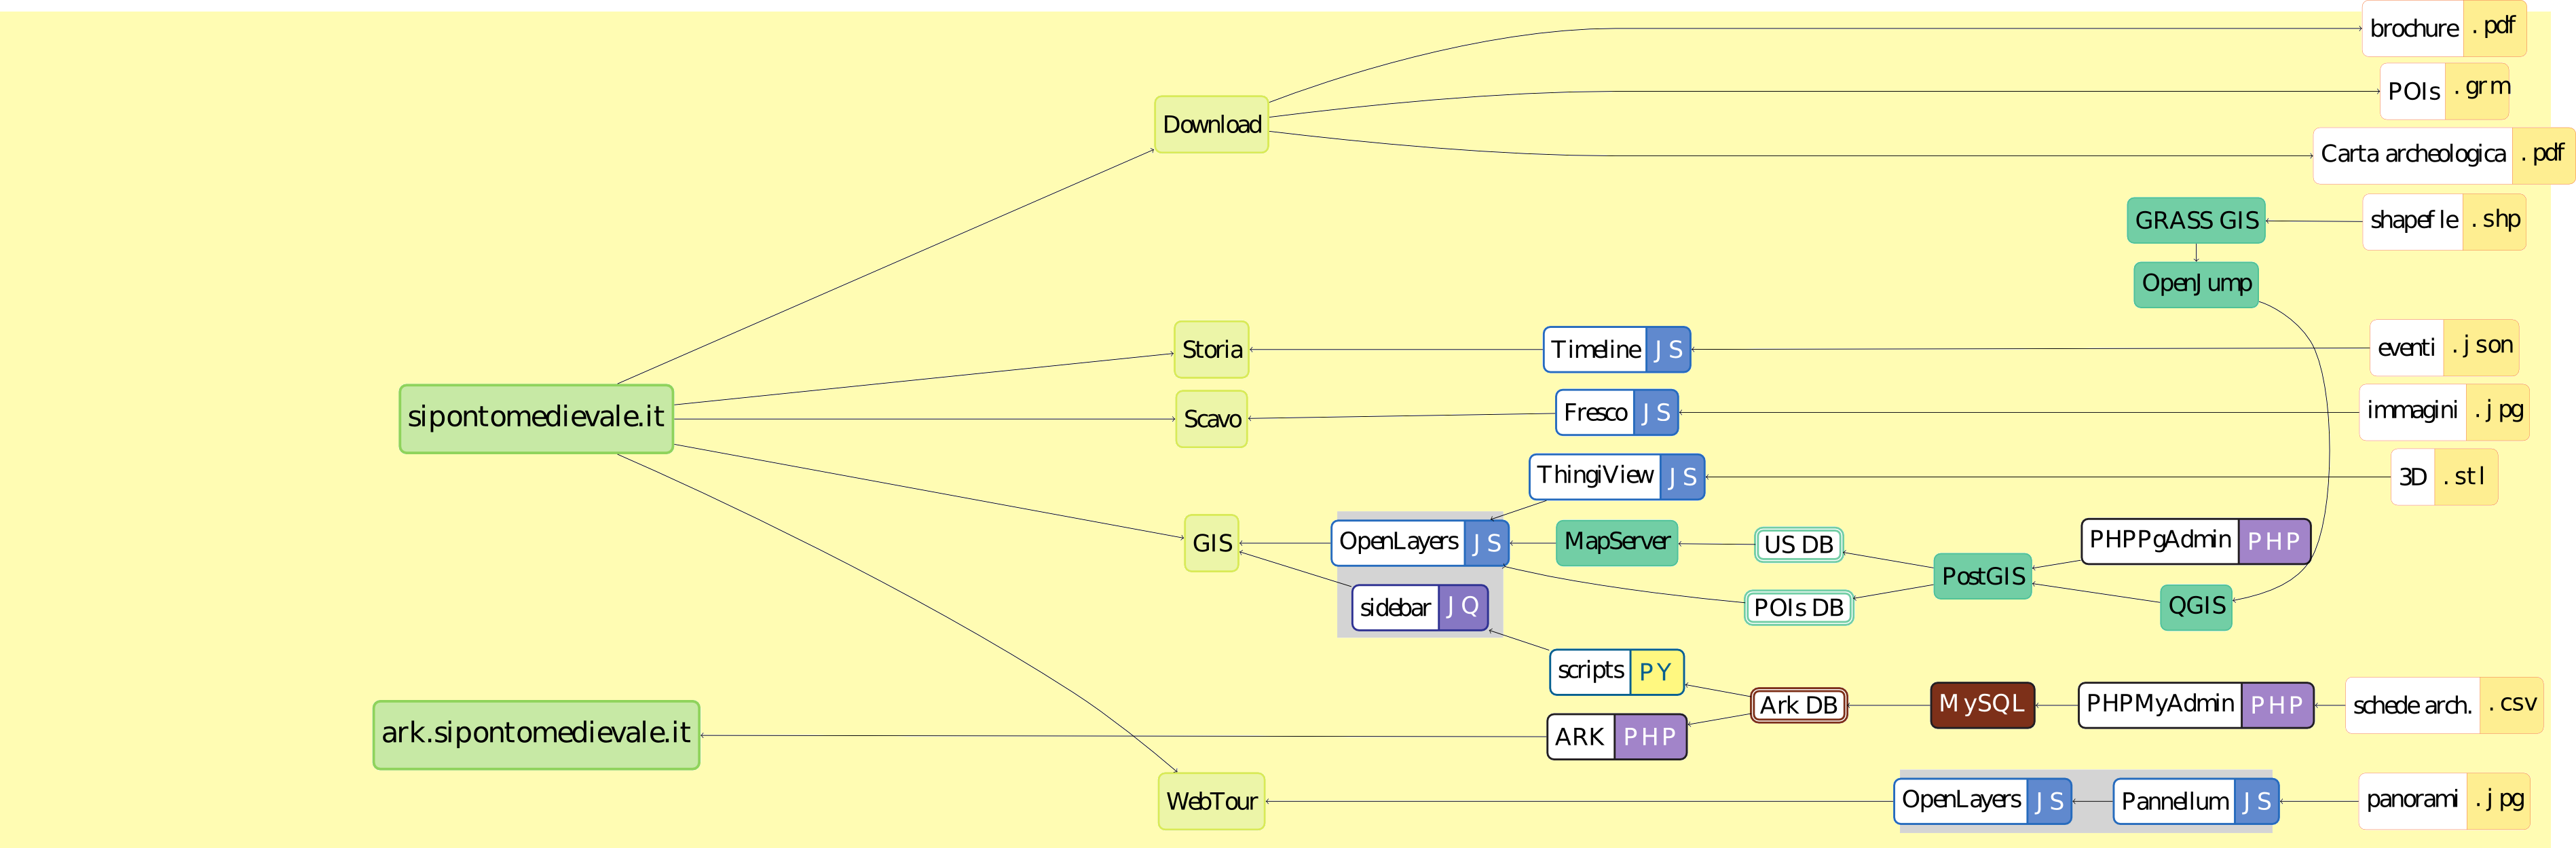
\includegraphics[width=0.85\textwidth]{scheme}
            \label{fig:scheme}
        \end{figure}
        \vspace{-0.5cm}
        %\resizebox{0.8\linewidth}{!}{
            %\begin{tikzpicture}[
                    %fill=black!20,
                    %main/.style
                        %={rectangle, draw=YellowGreen, ultra thick, fill=YellowGreen!50,
                        %text centered, rounded corners,
                        %minimum height=3em},
                    %page/.style
                        %={rectangle, draw=GreenYellow, very thick, fill=GreenYellow!50,
                        %text centered, rounded corners,
                        %minimum height=2.5em},
                    %file/.style
                        %={rectangle split,
                          %rectangle split horizontal,
                          %rectangle split parts=2,
                          %rectangle split part fill={White, Goldenrod!50},
                          %draw=Orange, very thin,
                          %text centered, rounded corners,
                          %minimum height=2.5em},
                    %js/.style
                        %={rectangle split,
                          %rectangle split horizontal,
                          %rectangle split parts=2,
                          %rectangle split part fill={White, NavyBlue!70},
                          %draw=NavyBlue, very thick,
                          %text centered, rounded corners,
                          %minimum height=2em},
                    %jquery/.style
                        %={rectangle split,
                          %rectangle split horizontal,
                          %rectangle split parts=2,
                          %rectangle split part fill={White, Blue!50},
                          %draw=Blue, very thick,
                          %text centered, rounded corners,
                          %minimum height=2em},
                    %php/.style
                        %={rectangle split,
                          %rectangle split horizontal,
                          %rectangle split parts=2,
                          %rectangle split part fill={White, RoyalPurple!50},
                          %draw=Black, very thick,
                          %text centered, rounded corners,
                          %minimum height=2em},
                    %py/.style
                        %={rectangle split,
                          %rectangle split horizontal,
                          %rectangle split parts=2,
                          %rectangle split part fill={White, Yellow!50},
                          %draw=MidnightBlue, very thick,
                          %text centered, rounded corners,
                          %minimum height=2em},
                    %gis/.style
                        %={rectangle, draw=SeaGreen, thick, fill=SeaGreen!80,
                        %text centered, rounded corners,
                        %minimum height=2em},
                    %geodb/.style
                        %={rectangle, fill=White,
                          %draw=SeaGreen!80, very thick, double,
                          %text centered, rounded corners,
                          %minimum height=1em},
                    %mysql/.style
                        %={rectangle, fill=Sepia!80,
                          %draw=Black, very thick,
                          %text centered, rounded corners,
                          %minimum height=2em},
                    %db/.style
                        %={rectangle, fill=White,
                          %draw=Sepia!80, very thick, double,
                          %text centered, rounded corners,
                          %minimum height=1em}
            %]
                %%%
\begin{scope}
  \pgfsetstrokecolor{black}
  \definecolor{strokecol}{rgb}{1.0,1.0,1.0};
  \pgfsetstrokecolor{strokecol}
  \definecolor{fillcol}{rgb}{1.0,1.0,1.0};
  \pgfsetfillcolor{fillcol}
  \filldraw (0bp,-1bp) -- (0bp,504bp) -- (1541bp,504bp) -- (1541bp,-1bp) -- cycle;
\end{scope}
\begin{scope}
  \pgfsetstrokecolor{black}
  \definecolor{strokecol}{rgb}{1.0,1.0,1.0};
  \pgfsetstrokecolor{strokecol}
  \definecolor{fillcol}{rgb}{1.0,1.0,1.0};
  \pgfsetfillcolor{fillcol}
  \filldraw (0bp,-1bp) -- (0bp,504bp) -- (1541bp,504bp) -- (1541bp,-1bp) -- cycle;
\end{scope}
\begin{scope}
  \pgfsetstrokecolor{black}
  \definecolor{strokecol}{rgb}{1.0,1.0,1.0};
  \pgfsetstrokecolor{strokecol}
  \definecolor{fillcol}{rgb}{1.0,1.0,1.0};
  \pgfsetfillcolor{fillcol}
  \filldraw (0bp,-1bp) -- (0bp,504bp) -- (1541bp,504bp) -- (1541bp,-1bp) -- cycle;
\end{scope}
\begin{scope}
  \pgfsetstrokecolor{black}
  \definecolor{strokecol}{rgb}{1.0,1.0,1.0};
  \pgfsetstrokecolor{strokecol}
  \definecolor{fillcol}{rgb}{1.0,1.0,1.0};
  \pgfsetfillcolor{fillcol}
  \filldraw (0bp,-1bp) -- (0bp,504bp) -- (1541bp,504bp) -- (1541bp,-1bp) -- cycle;
\end{scope}
\begin{scope}
  \pgfsetstrokecolor{black}
  \definecolor{strokecol}{rgb}{1.0,1.0,1.0};
  \pgfsetstrokecolor{strokecol}
  \definecolor{fillcol}{rgb}{1.0,1.0,1.0};
  \pgfsetfillcolor{fillcol}
  \filldraw (0bp,-1bp) -- (0bp,504bp) -- (1541bp,504bp) -- (1541bp,-1bp) -- cycle;
\end{scope}
\begin{scope}
  \pgfsetstrokecolor{black}
  \definecolor{strokecol}{rgb}{1.0,1.0,1.0};
  \pgfsetstrokecolor{strokecol}
  \definecolor{fillcol}{rgb}{1.0,1.0,1.0};
  \pgfsetfillcolor{fillcol}
  \filldraw (0bp,-1bp) -- (0bp,504bp) -- (1541bp,504bp) -- (1541bp,-1bp) -- cycle;
\end{scope}
\begin{scope}
  \pgfsetstrokecolor{black}
  \definecolor{strokecol}{rgb}{1.0,1.0,1.0};
  \pgfsetstrokecolor{strokecol}
  \definecolor{fillcol}{rgb}{1.0,1.0,1.0};
  \pgfsetfillcolor{fillcol}
  \filldraw (0bp,-1bp) -- (0bp,504bp) -- (1541bp,504bp) -- (1541bp,-1bp) -- cycle;
\end{scope}
\begin{scope}
  \pgfsetstrokecolor{black}
  \definecolor{strokecol}{rgb}{1.0,1.0,1.0};
  \pgfsetstrokecolor{strokecol}
  \definecolor{fillcol}{rgb}{1.0,1.0,1.0};
  \pgfsetfillcolor{fillcol}
  \filldraw (0bp,-1bp) -- (0bp,504bp) -- (1541bp,504bp) -- (1541bp,-1bp) -- cycle;
\end{scope}
\begin{scope}
  \pgfsetstrokecolor{black}
  \definecolor{strokecol}{rgb}{1.0,1.0,1.0};
  \pgfsetstrokecolor{strokecol}
  \definecolor{fillcol}{rgb}{1.0,1.0,1.0};
  \pgfsetfillcolor{fillcol}
  \filldraw (0bp,-1bp) -- (0bp,504bp) -- (1541bp,504bp) -- (1541bp,-1bp) -- cycle;
\end{scope}
\begin{scope}
  \pgfsetstrokecolor{black}
  \definecolor{strokecol}{rgb}{1.0,1.0,1.0};
  \pgfsetstrokecolor{strokecol}
  \definecolor{fillcol}{rgb}{1.0,1.0,1.0};
  \pgfsetfillcolor{fillcol}
  \filldraw (0bp,-1bp) -- (0bp,504bp) -- (1541bp,504bp) -- (1541bp,-1bp) -- cycle;
\end{scope}
\begin{scope}
  \pgfsetstrokecolor{black}
  \definecolor{strokecol}{rgb}{0.83,0.83,0.83};
  \pgfsetstrokecolor{strokecol}
  \definecolor{fillcol}{rgb}{0.83,0.83,0.83};
  \pgfsetfillcolor{fillcol}
  \filldraw (808bp,126bp) -- (808bp,202bp) -- (908bp,202bp) -- (908bp,126bp) -- cycle;
\end{scope}
\begin{scope}
  \pgfsetstrokecolor{black}
  \definecolor{strokecol}{rgb}{0.83,0.83,0.83};
  \pgfsetstrokecolor{strokecol}
  \definecolor{fillcol}{rgb}{0.83,0.83,0.83};
  \pgfsetfillcolor{fillcol}
  \filldraw (1148bp,8bp) -- (1148bp,46bp) -- (1373bp,46bp) -- (1373bp,8bp) -- cycle;
\end{scope}
  \node (phpmyadmin) at (1327bp,85bp) [draw,ellipse,php] {PHPMyAdmin\nodepart{two}\textbf{\color{White}PHP}};
  \node (storia) at (732bp,300bp) [draw,ellipse,page] {\Large Storia};
  \node (thingiview) at (977bp,223bp) [draw,ellipse,js] {ThingiView\nodepart{two}\textbf{\color{White}JS}};
  \node (timelinejs) at (977bp,300bp) [draw,ellipse,js] {Timeline\nodepart{two}\textbf{\color{White}JS}};
  \node (openlayers_gis) at (858bp,183bp) [draw,ellipse,js] {OpenLayers\nodepart{two}\textbf{\color{White}JS}};
  \node (cartaarch) at (1477bp,417bp) [draw,ellipse,file] {Carta archeologica\nodepart{two}\texttt{.pdf}};
  \node (phppgadmin) at (1327bp,184bp) [draw,ellipse,php] {PHPPgAdmin\nodepart{two}\textbf{\color{White}PHP}};
  \node (mysql) at (1198bp,85bp) [draw,ellipse,mysql] {\textbf{\color{White}MySQL}};
  \node (download) at (732bp,436bp) [draw,ellipse,page] {\Large Download};
  \node (home) at (324bp,258bp) [draw,ellipse,main] {\textbf{\LARGE www.sipontomedievale.it}};
  \node (ark) at (977bp,66bp) [draw,ellipse,php] {ARK\nodepart{two}\textbf{\color{White}PHP}};
  \node (openlayers_tour) at (1198bp,27bp) [draw,ellipse,js] {OpenLayers\nodepart{two}\textbf{\color{White}JS}};
  \node (sidebar) at (858bp,144bp) [draw,ellipse,jquery] {sidebar\nodepart{two}\textbf{\color{White}JQ}};
  \node (gis) at (732bp,183bp) [draw,ellipse,page] {\Large GIS};
  \node (img) at (1477bp,262bp) [draw,ellipse,file] {immagini\nodepart{two}\texttt{.jpg}};
  \node (qgis) at (1327bp,144bp) [draw,ellipse,gis] {QGIS};
  \node (pannellum) at (1327bp,27bp) [draw,ellipse,js] {Pannellum\nodepart{two}\textbf{\color{White}JS}};
  \node (arkweb) at (324bp,67bp) [draw,ellipse,main] {\textbf{\LARGE ark.sipontomedievale.it}};
  \node (pgsql) at (1198bp,163bp) [draw,ellipse,gis] {PostGIS};
  \node (json) at (1477bp,301bp) [draw,ellipse,file] {eventi\nodepart{two}\texttt{.json}};
  \node (csv) at (1477bp,85bp) [draw,ellipse,file] {schede arch.\nodepart{two}\texttt{.csv}};
  \node (panos) at (1477bp,27bp) [draw,ellipse,file] {panorami\nodepart{two}\texttt{.jpg}};
  \node (shp) at (1477bp,377bp) [draw,ellipse,file] {shapefile\nodepart{two}\texttt{.shp}};
  \node (openjump) at (1327bp,339bp) [draw,ellipse,gis] {OpenJump};
  \node (python) at (977bp,105bp) [draw,ellipse,py] {scripts\nodepart{two}\textbf{\color{MidnightBlue}PY}};
  \node (pois) at (1477bp,456bp) [draw,ellipse,file] {POIs\nodepart{two}\texttt{.grm}};
  \node (webtour) at (732bp,27bp) [draw,ellipse,page] {\Large WebTour};
  \node (brochure) at (1477bp,494bp) [draw,ellipse,file] {brochure\nodepart{two}\texttt{.pdf}};
  \node (schede) at (1087bp,85bp) [draw,ellipse,db] {Ark DB};
  \node (grass) at (1327bp,378bp) [draw,ellipse,gis] {GRASS GIS};
  \node (frescojs) at (977bp,262bp) [draw,ellipse,js] {Fresco\nodepart{two}\textbf{\color{White}JS}};
  \node (stl) at (1477bp,223bp) [draw,ellipse,file] {3D\nodepart{two}\texttt{.stl}};
  \node (us) at (1087bp,182bp) [draw,ellipse,geodb] {US DB};
  \node (poidb) at (1087bp,144bp) [draw,ellipse,geodb] {POIs DB};
  \node (mapserver) at (977bp,183bp) [draw,ellipse,gis] {MapServer};
  \node (scavo) at (732bp,258bp) [draw,ellipse,page] {\Large Scavo};
  \draw [->] (home) ..controls (504.48bp,224.84bp) and (640.95bp,199.63bp)  .. (gis);
  \draw [->] (frescojs) ..controls (911bp,260.93bp) and (823.21bp,259.48bp)  .. (scavo);
  \draw [->] (download) ..controls (801.63bp,462.72bp) and (894.46bp,494bp)  .. (976bp,494bp) .. controls (1199bp,494bp) and (1199bp,494bp)  .. (1199bp,494bp) .. controls (1282.9bp,494bp) and (1381bp,494bp)  .. (brochure);
  \draw [->] (openlayers_tour) ..controls (1072.6bp,27bp) and (881.47bp,27bp)  .. (webtour);
  \draw [->] (pgsql) ..controls (1156.3bp,170.1bp) and (1137.4bp,173.38bp)  .. (us);
  \draw [->] (download) ..controls (823.44bp,447.49bp) and (905.31bp,456bp)  .. (976bp,456bp) .. controls (1199bp,456bp) and (1199bp,456bp)  .. (1199bp,456bp) .. controls (1288.8bp,456bp) and (1395bp,456bp)  .. (pois);
  \draw [->] (img) ..controls (1353.3bp,262bp) and (1102.3bp,262bp)  .. (frescojs);
  \draw [->] (download) ..controls (823.94bp,425.04bp) and (905.54bp,417bp)  .. (976bp,417bp) .. controls (1199bp,417bp) and (1199bp,417bp)  .. (1199bp,417bp) .. controls (1268.7bp,417bp) and (1348.3bp,417bp)  .. (cartaarch);
  \draw [->] (openjump) ..controls (1371.4bp,327.23bp) and (1387.4bp,318.86bp)  .. (1396bp,305bp) .. controls (1411.4bp,280.05bp) and (1411.4bp,197.95bp)  .. (1396bp,173bp) .. controls (1388bp,160.1bp) and (1373bp,152.94bp)  .. (qgis);
  \draw [->] (home) ..controls (656.96bp,258bp) and (676.56bp,258bp)  .. (scavo);
  \draw [->] (sidebar) ..controls (816.24bp,156.82bp) and (784.19bp,166.9bp)  .. (gis);
  \draw [->] (pgsql) ..controls (1157.6bp,156.13bp) and (1140.6bp,153.17bp)  .. (poidb);
  \draw [->] (timelinejs) ..controls (900.9bp,300bp) and (821.19bp,300bp)  .. (storia);
  \draw [->] (python) ..controls (938.38bp,117.54bp) and (909.91bp,127.03bp)  .. (sidebar);
  \draw [->] (qgis) ..controls (1286.5bp,149.9bp) and (1258.4bp,154.11bp)  .. (pgsql);
  \draw [->] (shp) ..controls (1426.5bp,377.33bp) and (1402bp,377.5bp)  .. (grass);
  \draw [->] (phpmyadmin) ..controls (1264.2bp,85bp) and (1252.1bp,85bp)  .. (mysql);
  \draw [->] (mapserver) ..controls (929.74bp,183bp) and (919.67bp,183bp)  .. (openlayers_gis);
  \draw [->] (ark) ..controls (908.32bp,66.104bp) and (784.07bp,66.295bp)  .. (arkweb);
  \draw [->] (thingiview) ..controls (934.85bp,208.93bp) and (912.05bp,201.14bp)  .. (openlayers_gis);
  \draw [->] (pannellum) ..controls (1277bp,27bp) and (1263.1bp,27bp)  .. (openlayers_tour);
  \draw [->] (mysql) ..controls (1153.5bp,85bp) and (1139.7bp,85bp)  .. (schede);
  \draw [->] (poidb) ..controls (1024.9bp,149.7bp) and (976.99bp,155.12bp)  .. (936bp,163bp) .. controls (922.73bp,165.55bp) and (908.36bp,169.08bp)  .. (openlayers_gis);
  \draw [->] (stl) ..controls (1401.4bp,223bp) and (1138.7bp,223bp)  .. (thingiview);
  \draw [->] (schede) ..controls (1044.3bp,77.671bp) and (1023.6bp,74.019bp)  .. (ark);
  \draw [->] (csv) ..controls (1420.4bp,85bp) and (1403.9bp,85bp)  .. (phpmyadmin);
  \draw [->] (phppgadmin) ..controls (1271bp,174.91bp) and (1251.8bp,171.73bp)  .. (pgsql);
  \draw [->] (json) ..controls (1377.1bp,300.8bp) and (1120.4bp,300.29bp)  .. (timelinejs);
  \draw [->] (openlayers_gis) ..controls (799.53bp,183bp) and (780.24bp,183bp)  .. (gis);
  \draw [->] (home) ..controls (443.26bp,309.85bp) and (623.73bp,388.97bp)  .. (download);
  \draw [->] (us) ..controls (1049.5bp,182.34bp) and (1037.3bp,182.45bp)  .. (mapserver);
  \draw [->] (grass) ..controls (1327bp,365.73bp) and (1327bp,362.75bp)  .. (openjump);
  \draw [->] (home) ..controls (426.34bp,213.52bp) and (550.58bp,155.72bp)  .. (648bp,93bp) .. controls (670.41bp,78.572bp) and (694.02bp,59.357bp)  .. (webtour);
  \draw [->] (home) ..controls (549.14bp,281.19bp) and (640.63bp,290.65bp)  .. (storia);
  \draw [->] (schede) ..controls (1045.6bp,92.474bp) and (1026.4bp,96.032bp)  .. (python);
  \draw [->] (panos) ..controls (1422.8bp,27bp) and (1397bp,27bp)  .. (pannellum);
%

            %\end{tikzpicture}
        %}

        \tiny
        \begin{multicols}{2}[][]
            \begin{description}

                \item[migrazione~dati]

                    Le \textbf{schede di unità stratigrafica} sono state trascritte manualmente all'interno di fogli di calcolo usando LibreOffice Calc ed esportate nel formato CSV, successivamente importato in MySQL usando le funzionalità di PHPMyAdmin. Essendo il processo di importazione dei dati in ARK (versione 1.0 beta) poco documentato, ci si è avvalsi del supporto degli sviluppatori, operando anche alcune modifiche al file SQL che viene distribuito insieme al software. Si è messa a punto una guida con il file SQL corretto, disponibile nel repository GIT del progetto.

                    Le problematiche legate alla \textbf{documentazione grafica} in formato DWG (legate alla sua chiusura, alla natura non georeferenziata e non proiettata dei dati) sono state superate procedendo all'esporazione in DXF da AutoCAD (con l'aiuto del responsabile della documentazione grafica, la dott.ssa Raffaella Palombella), quindi alla georeferenziazione ed esportazione in \textit{shapefile} usando GRASS GIS ed alcuni script in Bash per automatizzare il processo. La pulizia e divisione delle geometrie è stata effettuata con OpenJump e il caricamento in PostGIS è stato operato attraverso l'interfaccia fornita da Quantum GIS.

                \item[struttura~del~sito]

                    Raggiungibile all'indirizzo \textbf{www.sipontoaperta.it}, il sito è servito da una macchina gestita da Ubuntu Server con LAMP. Il sito è stato realizzato con Twitter Bootstrap, apprezzato per la sua \emph{responsiveness} (il sito è fruibile da computer, tablet, smartphone) e per la compatibilità con quasi tutti i maggiori browser web. Tutto il codice del sito (con l'esclusione delle librerie esterne) è rilasciato su GitHub in licenza GPL v3. Tra le pagine più rilevanti:

                    \begin{description}
                        \item[Home] contiene uno \textit{slider} JavaScript con alcune immagini aeree del sito, e le informazioni principali su posizione, orari e fruibilità
                        \item[Storia] oltre ai contenuti testuali, è presente una linea temporale interattiva integrante una breve descrizione ed un'immagine per ogni evento della storia sipontina tra il 465 ed il 1620 d.C., realizzata con TimelineJS
                        \item[Webtour] contiene il tour immersivo in HTML5 realizzato con Pannellum (fig.~\ref{fig:webtour}). Le fotografie panoramiche sono state ottenute mediante unione di foto con Hugin. Attraverso vari punti di osservazione è possibile camminare nel parco archeologico, ottenere informazioni sulla porzione osservata mediante una casella di testo laterale. Con l'esclusione delle fotografie, tutti i dati sono conservati in una tabella PostGIS insieme a geometrie puntuali. Al \textit{webtour} è affiancata una carta in OpenLayers che permette il trascinamento del puntatore che indica la posizione attuale, per spostarsi all'interno del parco sul punto panoramico immediatamente più vicino alla posizione cliccata. La corretta esecuzione di HTML5 da parte del browser è assicurata da \emph{webgl-utils.js}, che mostra un \textit{popover} in caso il browser o la scheda grafica non supportino la tecnologia.
                    \end{description}

                \item[GIS]

                    La pagina \textbf{GIS} presenta una carta OpenLayers della zona garganica avente come \textit{layer} di base OpenStreetMap. Una barra dei pulsanti permette di selezionare i \textit{layer} geografici all'interno del \textit{database} PostGIS, serviti da MapServer tramite standard OGC WFS. Per ogni \textit{layer} sono state definite delle opzioni relative al comportamento dello zoom o di eventuali \textit{layer} di base che vanno a sostituirsi a quello di default per migliorare la leggibilità delle unità stratigrafiche. I \textit{layer} presentati comprendono due tipi di geometrie:

                    \vspace{-0.15cm}
                    \begin{description}
                        \item[poligoni] rappresentativi delle unità stratigrafiche; contenenti rispettivamente US, USM, USS (pulsanti mutuamente esclusivi);
                        \item[puntuali] contengono le informazioni su reperti e panorami, che danno accesso agli elementi multimediali ad essi relativi (foto panoramiche, modelli 3D).
                    \end{description}
                    
                    \vspace{-0.25cm}
                    Il click su una geometria tra quelle visualizzate apre un pannello laterale contenente informazioni estratte dinamicamente dal database MySQL delle schede US di ARK tramite \textit{script} in Python e \textit{templating} Jinja2. Ai \textit{layer} dei poligoni possono essere sovrapposti quelli puntuali degli elementi multimediali selezionabili dall'apposito menù a tendina; questi sono rappresentativi dei dieci reperti più importanti rinvenuti nello scavo e permettono di accedere ad una barra laterale e ad un \emph{canvas} HTML5 (fig.~\ref{fig:gis}).

                \item[modelli~3D]

                    Selezionati tra i reperti ceramici, metallici, osteologici umani e animali, sono stati puliti e scansionati, ottenendo file STL. Sono stati superati i problemi legati alla riflessione operata dalle superfici metalliche, alle dimensioni ridotte di alcuni oggetti e al montaggio delle nuvole di reperti dalla struttura complessa. L'integrazione all'interno del webGIS è stata operata tramite Thingiview.js: gli STL vengono visualizzati dinamicamente all'interno di un \textit{canvas}, con il quale l'utente può interagire (zoom, rotazione, visualizzazione delle superfici o \textit{wireframe}).

                \item[interfaccia~ARK]

                    In un dominio di secondo livello del progetto, \emph{http://ark.sipontomedievale.it}, è raggiungibile l'interfaccia di accesso ad ARK che consente la gestione dei dati delle schede di US (fig.~\ref{fig:ark}): chiunque sia in possesso di credenziali può accedere ai dati via internet. L'interfaccia, seppure in lingua inglese, è di facile comprensione, e racchiude schede con funzioni specifiche per la gestione degli utenti, inserimento dati, lettura delle schede, ricerca avanzata, visualizzazione della carta, importazione dati.
        
            \end{description}
        \end{multicols}

        \vspace{-0.5cm}

        \begin{figure}[H]
            \minipage{0.32\textwidth}
                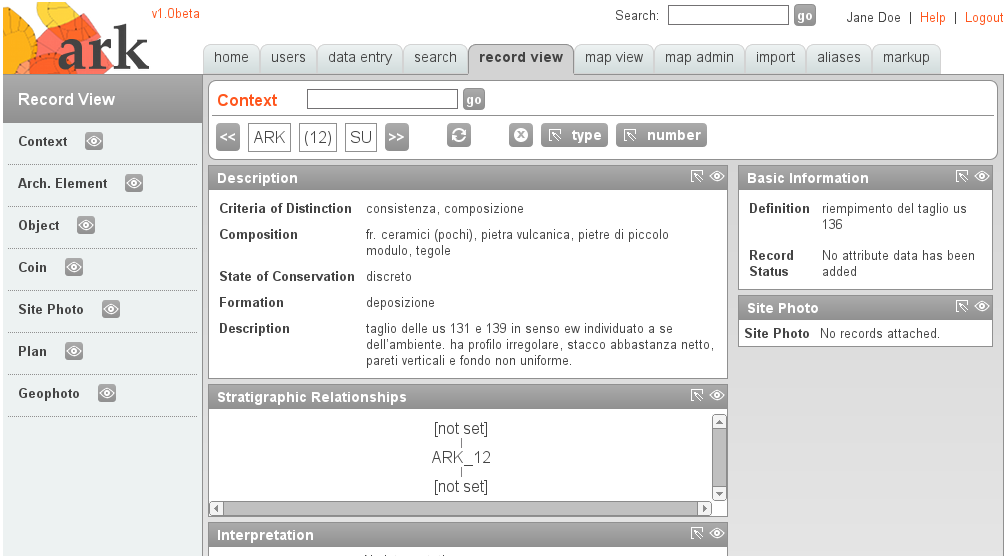
\includegraphics[width=\linewidth]{ark}
                \caption[]{Una scheda US in ARK.}\label{fig:ark}
            \endminipage\hfill
            \minipage{0.22\textwidth}
                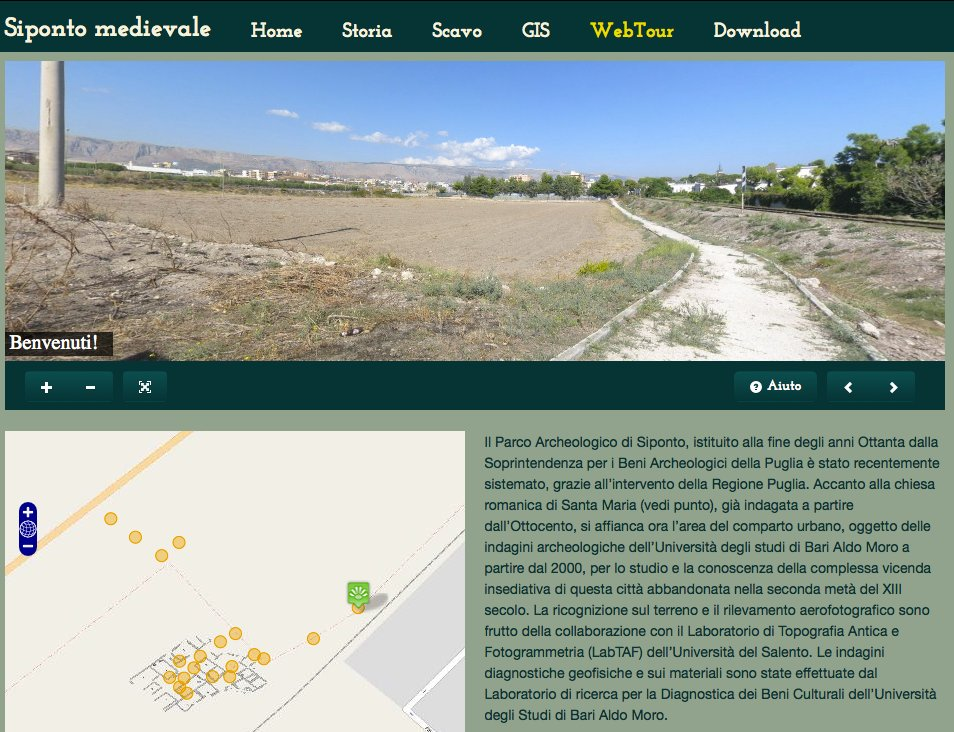
\includegraphics[width=\linewidth]{webtour}
                \caption[]{Webtour HTML5.}\label{fig:webtour}
            \endminipage\hfill
            \minipage{0.32\textwidth}
                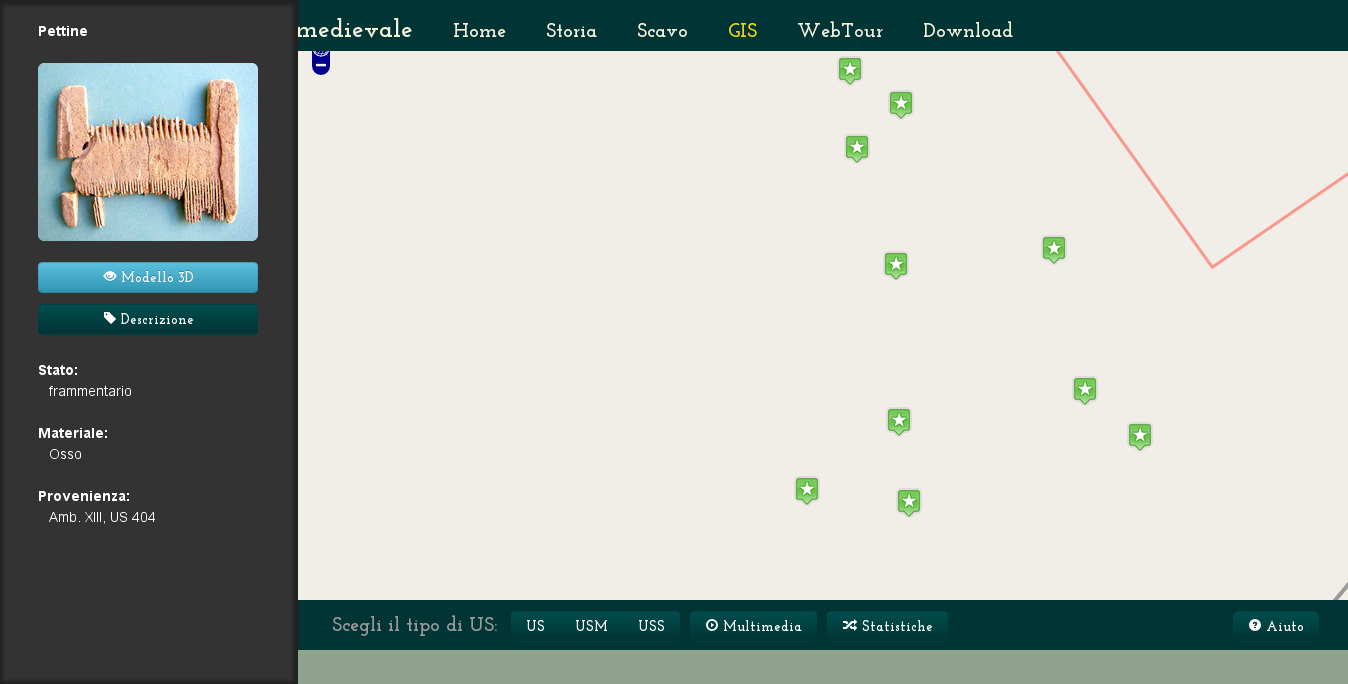
\includegraphics[width=\linewidth]{gis}
                \caption[]{WebGIS: pannello dei reperti 3D.}\label{fig:gis}
            \endminipage\hfill
        \end{figure}

        %\vspace{0.3em}
    }

    %%%%%%%%%%%%%%%%%%%%%%%%%%%%%%%%%%%%%%%%%%%%%%%%%%%%%%%%%%%%%%%%%%%%%%%%%%%%%%
    \headerbox{Conclusioni}{name=conclusioni,column=1,span=2,below=specifics}{\scriptsize
    %%%%%%%%%%%%%%%%%%%%%%%%%%%%%%%%%%%%%%%%%%%%%%%%%%%%%%%%%%%%%%%%%%%%%%%%%%%%%%

        I vantaggi dell'approccio descritto rispetto alla gestione tradizionale dello scavo sono tanto maggiori quanto maggiore è il volume dei dati da trattare, e discendono in parte dalla qualità del software utilizzato ed in parte dalla modularità e dall'adozione di standard nella comunicazione tra i vari componenti (tra tutti, il WFS). L'implementazione di altre componenti amplierebbe ulteriormente i vantaggi elencati:

        \begin{itemize}
            \itemsep0em
            \item migrazione del database di ARK da MySQL a PostGIS con integrazione dei dati geografici; strumenti per l'importazione diretta dei CSV in ARK;
            \item sistema di pacchettizzazione che renda semplice l'installazione degli applicativi (in particolare ARK) su macchine \textit{destkop}/\textit{server} ed integrazione con distribuzioni \textit{software} orientate all'archeologia (tra tutte, ricordiamo ArcheOS);
            \item integrare un sistema di API in ARK permetterebbe l'interrogazione selettiva e l'esporazione verso sistemi più ampi (tra tutti, verso i nuovi sistemi informativi archeologici italiani --- SITAR);
            \item interfaccia web per la rapida configurazione di un \textit{webtour} immersivo;
        \end{itemize}

        %\vspace{0.3em}
    }

    %%%%%%%%%%%%%%%%%%%%%%%%%%%%%%%%%%%%%%%%%%%%%%%%%%%%%%%%%%%%%%%%%%%%%%%%%%%%%%
    \headerbox{Bibliografia}{name=references,column=0,below=project}{
    %%%%%%%%%%%%%%%%%%%%%%%%%%%%%%%%%%%%%%%%%%%%%%%%%%%%%%%%%%%%%%%%%%%%%%%%%%%%%%

        \vspace{-0.4em}

        \renewcommand*{\bibfont}{\scriptsize}
        \renewcommand{\section}[2]{\vskip 0.3em}
        \printbibliography

        \textbf{\scriptsize{Quest'opera è rilasciata con licenza Creative Commons CC-BY-SA
        \begin{center}
            \cc\ccby\ccsa
        \end{center}}}
    }

\end{poster}
\end{document}
